\documentclass[]{article}
\usepackage{lmodern}
\usepackage{amssymb,amsmath}
\usepackage{ifxetex,ifluatex}
\usepackage{fixltx2e} % provides \textsubscript
\ifnum 0\ifxetex 1\fi\ifluatex 1\fi=0 % if pdftex
  \usepackage[T1]{fontenc}
  \usepackage[utf8]{inputenc}
\else % if luatex or xelatex
  \ifxetex
    \usepackage{mathspec}
  \else
    \usepackage{fontspec}
  \fi
  \defaultfontfeatures{Ligatures=TeX,Scale=MatchLowercase}
\fi
% use upquote if available, for straight quotes in verbatim environments
\IfFileExists{upquote.sty}{\usepackage{upquote}}{}
% use microtype if available
\IfFileExists{microtype.sty}{%
\usepackage{microtype}
\UseMicrotypeSet[protrusion]{basicmath} % disable protrusion for tt fonts
}{}
\usepackage[margin=1in]{geometry}
\usepackage{hyperref}
\hypersetup{unicode=true,
            pdftitle={Regresion},
            pdfborder={0 0 0},
            breaklinks=true}
\urlstyle{same}  % don't use monospace font for urls
\usepackage{color}
\usepackage{fancyvrb}
\newcommand{\VerbBar}{|}
\newcommand{\VERB}{\Verb[commandchars=\\\{\}]}
\DefineVerbatimEnvironment{Highlighting}{Verbatim}{commandchars=\\\{\}}
% Add ',fontsize=\small' for more characters per line
\usepackage{framed}
\definecolor{shadecolor}{RGB}{248,248,248}
\newenvironment{Shaded}{\begin{snugshade}}{\end{snugshade}}
\newcommand{\AlertTok}[1]{\textcolor[rgb]{0.94,0.16,0.16}{#1}}
\newcommand{\AnnotationTok}[1]{\textcolor[rgb]{0.56,0.35,0.01}{\textbf{\textit{#1}}}}
\newcommand{\AttributeTok}[1]{\textcolor[rgb]{0.77,0.63,0.00}{#1}}
\newcommand{\BaseNTok}[1]{\textcolor[rgb]{0.00,0.00,0.81}{#1}}
\newcommand{\BuiltInTok}[1]{#1}
\newcommand{\CharTok}[1]{\textcolor[rgb]{0.31,0.60,0.02}{#1}}
\newcommand{\CommentTok}[1]{\textcolor[rgb]{0.56,0.35,0.01}{\textit{#1}}}
\newcommand{\CommentVarTok}[1]{\textcolor[rgb]{0.56,0.35,0.01}{\textbf{\textit{#1}}}}
\newcommand{\ConstantTok}[1]{\textcolor[rgb]{0.00,0.00,0.00}{#1}}
\newcommand{\ControlFlowTok}[1]{\textcolor[rgb]{0.13,0.29,0.53}{\textbf{#1}}}
\newcommand{\DataTypeTok}[1]{\textcolor[rgb]{0.13,0.29,0.53}{#1}}
\newcommand{\DecValTok}[1]{\textcolor[rgb]{0.00,0.00,0.81}{#1}}
\newcommand{\DocumentationTok}[1]{\textcolor[rgb]{0.56,0.35,0.01}{\textbf{\textit{#1}}}}
\newcommand{\ErrorTok}[1]{\textcolor[rgb]{0.64,0.00,0.00}{\textbf{#1}}}
\newcommand{\ExtensionTok}[1]{#1}
\newcommand{\FloatTok}[1]{\textcolor[rgb]{0.00,0.00,0.81}{#1}}
\newcommand{\FunctionTok}[1]{\textcolor[rgb]{0.00,0.00,0.00}{#1}}
\newcommand{\ImportTok}[1]{#1}
\newcommand{\InformationTok}[1]{\textcolor[rgb]{0.56,0.35,0.01}{\textbf{\textit{#1}}}}
\newcommand{\KeywordTok}[1]{\textcolor[rgb]{0.13,0.29,0.53}{\textbf{#1}}}
\newcommand{\NormalTok}[1]{#1}
\newcommand{\OperatorTok}[1]{\textcolor[rgb]{0.81,0.36,0.00}{\textbf{#1}}}
\newcommand{\OtherTok}[1]{\textcolor[rgb]{0.56,0.35,0.01}{#1}}
\newcommand{\PreprocessorTok}[1]{\textcolor[rgb]{0.56,0.35,0.01}{\textit{#1}}}
\newcommand{\RegionMarkerTok}[1]{#1}
\newcommand{\SpecialCharTok}[1]{\textcolor[rgb]{0.00,0.00,0.00}{#1}}
\newcommand{\SpecialStringTok}[1]{\textcolor[rgb]{0.31,0.60,0.02}{#1}}
\newcommand{\StringTok}[1]{\textcolor[rgb]{0.31,0.60,0.02}{#1}}
\newcommand{\VariableTok}[1]{\textcolor[rgb]{0.00,0.00,0.00}{#1}}
\newcommand{\VerbatimStringTok}[1]{\textcolor[rgb]{0.31,0.60,0.02}{#1}}
\newcommand{\WarningTok}[1]{\textcolor[rgb]{0.56,0.35,0.01}{\textbf{\textit{#1}}}}
\usepackage{graphicx,grffile}
\makeatletter
\def\maxwidth{\ifdim\Gin@nat@width>\linewidth\linewidth\else\Gin@nat@width\fi}
\def\maxheight{\ifdim\Gin@nat@height>\textheight\textheight\else\Gin@nat@height\fi}
\makeatother
% Scale images if necessary, so that they will not overflow the page
% margins by default, and it is still possible to overwrite the defaults
% using explicit options in \includegraphics[width, height, ...]{}
\setkeys{Gin}{width=\maxwidth,height=\maxheight,keepaspectratio}
\IfFileExists{parskip.sty}{%
\usepackage{parskip}
}{% else
\setlength{\parindent}{0pt}
\setlength{\parskip}{6pt plus 2pt minus 1pt}
}
\setlength{\emergencystretch}{3em}  % prevent overfull lines
\providecommand{\tightlist}{%
  \setlength{\itemsep}{0pt}\setlength{\parskip}{0pt}}
\setcounter{secnumdepth}{0}
% Redefines (sub)paragraphs to behave more like sections
\ifx\paragraph\undefined\else
\let\oldparagraph\paragraph
\renewcommand{\paragraph}[1]{\oldparagraph{#1}\mbox{}}
\fi
\ifx\subparagraph\undefined\else
\let\oldsubparagraph\subparagraph
\renewcommand{\subparagraph}[1]{\oldsubparagraph{#1}\mbox{}}
\fi

%%% Use protect on footnotes to avoid problems with footnotes in titles
\let\rmarkdownfootnote\footnote%
\def\footnote{\protect\rmarkdownfootnote}

%%% Change title format to be more compact
\usepackage{titling}

% Create subtitle command for use in maketitle
\providecommand{\subtitle}[1]{
  \posttitle{
    \begin{center}\large#1\end{center}
    }
}

\setlength{\droptitle}{-2em}

  \title{Regresion}
    \pretitle{\vspace{\droptitle}\centering\huge}
  \posttitle{\par}
    \author{}
    \preauthor{}\postauthor{}
    \date{}
    \predate{}\postdate{}
  

\begin{document}
\maketitle

\hypertarget{tarea-3.}{%
\section{Tarea 3.}\label{tarea-3.}}

\hypertarget{regresion-lineal}{%
\section{Regresión lineal}\label{regresion-lineal}}

\hypertarget{jorge-porras-araya}{%
\section{Jorge Porras Araya}\label{jorge-porras-araya}}

Análisis del Problema

El desempeño de un automóvil se puede medir de diferentes formas.
Algunas comunes son la cantidad de caballos de fuerza y el rendimiento
del mismo, que se puede resumir en cuantas millas puede recorrer el
automóvil por cada galón de combustible que consume. Para los clientes,
potenciales compradores de un automóvil, este rendimiento es importante
pues puede ayudar a tomar una decisión con respecto a cuál automóvil
comprar (si, por ejemplo, el cliente quiere un auto que rinda por muchas
millas y pueda economizar en la compra de combustible).

Desde este punto de vista, tanto a clientes como a fabricadores de
automóviles, les conviene entender cuál es la relación entre diferentes
características del automóvil y su rendimiento, pues el conocer estas
relaciones les puede ayudar a inferir cuál va a ser la eficiencia del
vehículo a partir de ver los valores de otras características. Para
fabricantes, puede ser importante conocer estas relaciones para saber
cómo hacer cada modelo más eficiente con respecto al anterior.

Entendimiento de los Datos

Con el fin de analizar y tratar de estimar las millas por galón de
diferentes modelos de automóviles, se trabajó con un conjunto de datos
que contiene 398 observaciones y 9 variables:

\begin{itemize}
\tightlist
\item
  mpg (millas por galón): numérica, con un rango de 9 a 46.60.
\item
  cyl (cilindraje): categórica ordinal, con valores posibles de 3, 4, 5,
  6 y 8.
\item
  disp (desplazamiento): numérica, con un rango de 68 a 455.
\item
  hp (caballos de fuerza): numérica, con un rango de 46 a 230 y 6
  valores faltantes.
\item
  weight (peso): numérica, con un rango de 1613 a 5140.
\item
  acc (aceleración): numérica, con un rango de 8 a 24.80.
\item
  model year (año): categórica, con 13 valores diferentes representando
  el año del automóvil.
\item
  origin (origen): categórica, 3 valores posibles: 1, 2, 3.
\item
  model name (nombre del modelo): categórica, con 305 posibles valores.
\end{itemize}

\hypertarget{ejercicios}{%
\section{Ejercicios}\label{ejercicios}}

\hypertarget{prueba-1}{%
\section{Prueba 1}\label{prueba-1}}

\begin{enumerate}
\def\labelenumi{\arabic{enumi}.}
\tightlist
\item
  Cargue el archivo auto-mpg\_g.csv en una variable
\end{enumerate}

\begin{Shaded}
\begin{Highlighting}[]
  \KeywordTok{library}\NormalTok{(GGally)}
\end{Highlighting}
\end{Shaded}

\begin{verbatim}
## Warning: package 'GGally' was built under R version 3.6.1
\end{verbatim}

\begin{verbatim}
## Loading required package: ggplot2
\end{verbatim}

\begin{verbatim}
## Registered S3 method overwritten by 'GGally':
##   method from   
##   +.gg   ggplot2
\end{verbatim}

\begin{Shaded}
\begin{Highlighting}[]
  \KeywordTok{library}\NormalTok{(MASS)}
  \KeywordTok{library}\NormalTok{(caTools)}
  \KeywordTok{library}\NormalTok{(visdat)}
\end{Highlighting}
\end{Shaded}

\begin{verbatim}
## Warning: package 'visdat' was built under R version 3.6.1
\end{verbatim}

\begin{Shaded}
\begin{Highlighting}[]
  \KeywordTok{library}\NormalTok{(Metrics)}
\end{Highlighting}
\end{Shaded}

\begin{verbatim}
## Warning: package 'Metrics' was built under R version 3.6.1
\end{verbatim}

\begin{Shaded}
\begin{Highlighting}[]
  \KeywordTok{library}\NormalTok{(dplyr)}
\end{Highlighting}
\end{Shaded}

\begin{verbatim}
## 
## Attaching package: 'dplyr'
\end{verbatim}

\begin{verbatim}
## The following object is masked from 'package:MASS':
## 
##     select
\end{verbatim}

\begin{verbatim}
## The following object is masked from 'package:GGally':
## 
##     nasa
\end{verbatim}

\begin{verbatim}
## The following objects are masked from 'package:stats':
## 
##     filter, lag
\end{verbatim}

\begin{verbatim}
## The following objects are masked from 'package:base':
## 
##     intersect, setdiff, setequal, union
\end{verbatim}

Se lee el archivo .csv la visualizacion de los datos nos muestra que no
tenemos valores nulos model.name es un factor Se guardan los valores de
los modelos de los vehiculos Se eliminan las variables categoricas Se
eliminan las filas con hp = 0, pues si se desea emplear escala
logaritmica, log(0) esta indefinido (-inf), ademas no pueden existir
vehiculos con potencia = 0hp

\begin{Shaded}
\begin{Highlighting}[]
\NormalTok{  autosCSV <-}\StringTok{ }\KeywordTok{read.csv}\NormalTok{(}\StringTok{"auto-mpg_g.csv"}\NormalTok{)}
\NormalTok{  autos <-}\StringTok{ }\NormalTok{autosCSV }\OperatorTok\StringTok{ }
\StringTok{    }\KeywordTok{select}\NormalTok{ (mpg, disp, hp, weight, acc, model.name) }\OperatorTok\StringTok{ }
\StringTok{    }\KeywordTok{filter}\NormalTok{(hp }\OperatorTok{>}\StringTok{ }\DecValTok{0}\NormalTok{)}

  \KeywordTok{vis_dat}\NormalTok{(autos)}
\end{Highlighting}
\end{Shaded}

\includegraphics{Regresion_files/figure-latex/unnamed-chunk-2-1.pdf}

\begin{Shaded}
\begin{Highlighting}[]
\NormalTok{  Y <-}\StringTok{ }\NormalTok{autos }\OperatorTok\StringTok{ }\KeywordTok{select}\NormalTok{(model.name)       }\CommentTok{#Etiquetas  }
\end{Highlighting}
\end{Shaded}

\begin{Shaded}
\begin{Highlighting}[]
\KeywordTok{boxplot}\NormalTok{(autos}\OperatorTok{$}\NormalTok{mpg, }
        \DataTypeTok{main=}\StringTok{"Consumo de combustible"}\NormalTok{,}
        \DataTypeTok{ylab=}\StringTok{"mpg"}\NormalTok{)}
\end{Highlighting}
\end{Shaded}

\includegraphics{Regresion_files/figure-latex/unnamed-chunk-3-1.pdf}

\begin{Shaded}
\begin{Highlighting}[]
\KeywordTok{boxplot}\NormalTok{(autos}\OperatorTok{$}\NormalTok{hp, }
        \DataTypeTok{main=}\StringTok{"Potencia"}\NormalTok{,}
        \DataTypeTok{ylab=}\StringTok{"hp"}\NormalTok{)}
\end{Highlighting}
\end{Shaded}

\includegraphics{Regresion_files/figure-latex/unnamed-chunk-3-2.pdf}

\begin{Shaded}
\begin{Highlighting}[]
\KeywordTok{boxplot}\NormalTok{(autos}\OperatorTok{$}\NormalTok{weight, }
        \DataTypeTok{main=}\StringTok{"Peso"}\NormalTok{,}
        \DataTypeTok{ylab=}\StringTok{"pounds"}\NormalTok{)}
\end{Highlighting}
\end{Shaded}

\includegraphics{Regresion_files/figure-latex/unnamed-chunk-3-3.pdf}

de los histogramas se puede observar que existen algunos puntos en hp
que son considerados outliers, sin embargo se decide no eliminarlos pues
son valores reales de potencia de vehiculos.

\begin{Shaded}
\begin{Highlighting}[]
\NormalTok{outliers <-}\StringTok{ }\KeywordTok{boxplot}\NormalTok{(autos}\OperatorTok{$}\NormalTok{hp, }\DataTypeTok{plot =}\NormalTok{ F)}\OperatorTok{$}\NormalTok{out}
\NormalTok{outliers}
\end{Highlighting}
\end{Shaded}

\begin{verbatim}
##  [1] 220 215 225 225 215 210 208 215 225 230
\end{verbatim}

\begin{enumerate}
\def\labelenumi{\arabic{enumi}.}
\setcounter{enumi}{1}
\tightlist
\item
  Utilizando Ggpairs cree un gráfico de los atributos del dataset,
  observe las correlaciones entre atributos
\end{enumerate}

\begin{Shaded}
\begin{Highlighting}[]
\CommentTok{# ggpairs(autos, progress = F)}
\end{Highlighting}
\end{Shaded}

\begin{enumerate}
\def\labelenumi{\arabic{enumi}.}
\setcounter{enumi}{2}
\tightlist
\item
  Separe los datos en 2 conjuntos, uno de entrenamiento y otro de
  pruebas. Normalmente se trabaja utilizando un 70-80\% de los datos
  para entrenamiento y el resto para pruebas.
\end{enumerate}

Recuerde fijar una semilla para que el documento sea reproducible.

Pista:
\url{https://www.rdocumentation.org/packages/caTools/versions/1.17.1/topics/sample.split}

\begin{Shaded}
\begin{Highlighting}[]
  \KeywordTok{set.seed}\NormalTok{(}\DecValTok{4}\NormalTok{)}
\NormalTok{  mask <-}\StringTok{ }\KeywordTok{sample.split}\NormalTok{(Y}\OperatorTok{$}\NormalTok{model.name, }\DataTypeTok{SplitRatio =} \DecValTok{7}\OperatorTok{/}\DecValTok{10}\NormalTok{)}
\NormalTok{  training_data <-}\StringTok{ }\NormalTok{autos[mask, }\KeywordTok{c}\NormalTok{(}\DecValTok{1}\NormalTok{, }\DecValTok{2}\NormalTok{, }\DecValTok{3}\NormalTok{, }\DecValTok{4}\NormalTok{)]}
\NormalTok{  test_data <-}\StringTok{ }\NormalTok{autos[}\OperatorTok{!}\NormalTok{mask, }\KeywordTok{c}\NormalTok{(}\DecValTok{1}\NormalTok{, }\DecValTok{2}\NormalTok{, }\DecValTok{3}\NormalTok{, }\DecValTok{4}\NormalTok{)]}

\KeywordTok{tail}\NormalTok{(training_data, }\DecValTok{10}\NormalTok{)}
\end{Highlighting}
\end{Shaded}

\begin{verbatim}
##     mpg disp  hp weight
## 379  32   91  67   1965
## 380  38   91  67   1995
## 381  25  181 110   2945
## 383  26  156  92   2585
## 387  27  151  90   2950
## 388  27  140  86   2790
## 389  44   97  52   2130
## 390  32  135  84   2295
## 391  28  120  79   2625
## 392  31  119  82   2720
\end{verbatim}

revisando la relacion entre los datos de entrenamiento y los de prueba
se puede observar que la relacion es de aproximadamente 70\%, el cual es
el valor esperado.

\begin{Shaded}
\begin{Highlighting}[]
\NormalTok{  ratio <-}\StringTok{ }\DecValTok{100} \OperatorTok{*}\StringTok{ }\KeywordTok{length}\NormalTok{(training_data}\OperatorTok{$}\NormalTok{mpg) }\OperatorTok{/}
\StringTok{    }\NormalTok{(}\KeywordTok{length}\NormalTok{(training_data}\OperatorTok{$}\NormalTok{mpg) }\OperatorTok{+}\StringTok{ }\KeywordTok{length}\NormalTok{(test_data}\OperatorTok{$}\NormalTok{mpg))}
  
\NormalTok{ratio}
\end{Highlighting}
\end{Shaded}

\begin{verbatim}
## [1] 69.89796
\end{verbatim}

utilizando como variable objetivo mpg y como variables predictoras disp
y weight, se realiza un histograma para observar el comportamiento de
las variables

\begin{Shaded}
\begin{Highlighting}[]
\KeywordTok{hist}\NormalTok{(training_data}\OperatorTok{$}\NormalTok{mpg)}
\end{Highlighting}
\end{Shaded}

\includegraphics{Regresion_files/figure-latex/unnamed-chunk-8-1.pdf}

\begin{Shaded}
\begin{Highlighting}[]
\KeywordTok{hist}\NormalTok{(training_data}\OperatorTok{$}\NormalTok{hp)}
\end{Highlighting}
\end{Shaded}

\includegraphics{Regresion_files/figure-latex/unnamed-chunk-8-2.pdf}

\begin{Shaded}
\begin{Highlighting}[]
\KeywordTok{hist}\NormalTok{(training_data}\OperatorTok{$}\NormalTok{weight)}
\end{Highlighting}
\end{Shaded}

\includegraphics{Regresion_files/figure-latex/unnamed-chunk-8-3.pdf}

\begin{Shaded}
\begin{Highlighting}[]
\KeywordTok{hist}\NormalTok{(training_data}\OperatorTok{$}\NormalTok{disp)}
\end{Highlighting}
\end{Shaded}

\includegraphics{Regresion_files/figure-latex/unnamed-chunk-8-4.pdf}

\begin{Shaded}
\begin{Highlighting}[]
\KeywordTok{hist}\NormalTok{(}\KeywordTok{log}\NormalTok{(training_data}\OperatorTok{$}\NormalTok{mpg))}
\end{Highlighting}
\end{Shaded}

\includegraphics{Regresion_files/figure-latex/unnamed-chunk-9-1.pdf}

\begin{Shaded}
\begin{Highlighting}[]
\KeywordTok{hist}\NormalTok{(}\KeywordTok{log}\NormalTok{(training_data}\OperatorTok{$}\NormalTok{hp))}
\end{Highlighting}
\end{Shaded}

\includegraphics{Regresion_files/figure-latex/unnamed-chunk-9-2.pdf}

\begin{Shaded}
\begin{Highlighting}[]
\KeywordTok{hist}\NormalTok{(}\KeywordTok{log}\NormalTok{(training_data}\OperatorTok{$}\NormalTok{weight))}
\end{Highlighting}
\end{Shaded}

\includegraphics{Regresion_files/figure-latex/unnamed-chunk-9-3.pdf}

\begin{Shaded}
\begin{Highlighting}[]
\KeywordTok{hist}\NormalTok{(}\KeywordTok{log}\NormalTok{(training_data}\OperatorTok{$}\NormalTok{disp))}
\end{Highlighting}
\end{Shaded}

\includegraphics{Regresion_files/figure-latex/unnamed-chunk-9-4.pdf}

\begin{Shaded}
\begin{Highlighting}[]
  \KeywordTok{plot}\NormalTok{(training_data}\OperatorTok{$}\NormalTok{hp, training_data}\OperatorTok{$}\NormalTok{mpg)}
\end{Highlighting}
\end{Shaded}

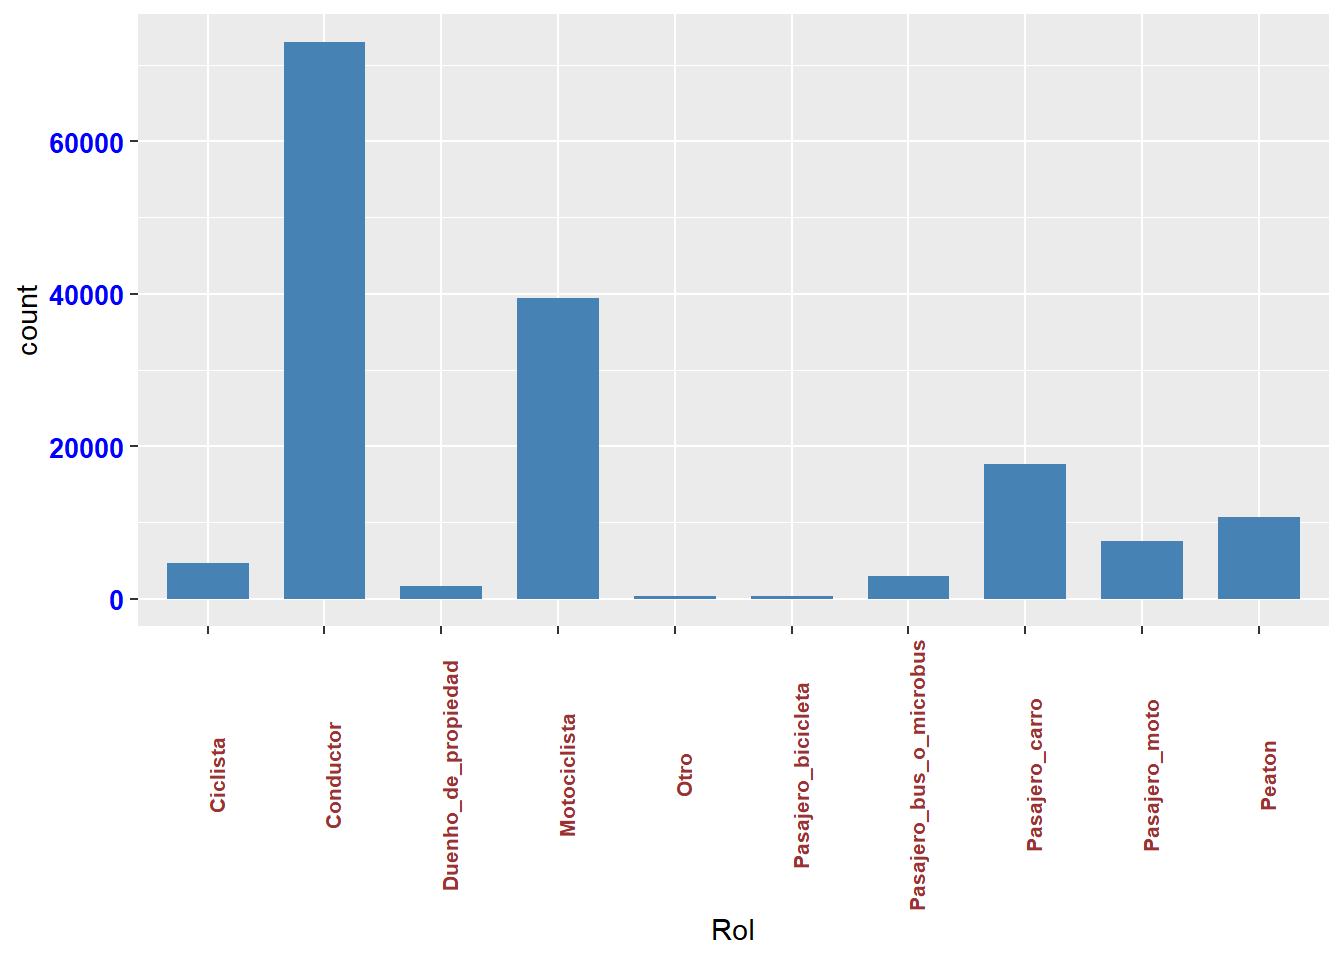
\includegraphics{Regresion_files/figure-latex/unnamed-chunk-10-1.pdf}

\begin{Shaded}
\begin{Highlighting}[]
  \KeywordTok{plot}\NormalTok{(training_data}\OperatorTok{$}\NormalTok{weight, training_data}\OperatorTok{$}\NormalTok{mpg)}
\end{Highlighting}
\end{Shaded}

\includegraphics{Regresion_files/figure-latex/unnamed-chunk-11-1.pdf}

\begin{enumerate}
\def\labelenumi{\arabic{enumi}.}
\setcounter{enumi}{3}
\tightlist
\item
  Cree un modelo de regresion lineal utilizando el atributo mpg como la
  variable objetivo y en base a las correlaciones observadas en el
  gráfico del punto 2 escoja al menos dos atributos para usarlos como
  variables predictoras para el modelo.
\end{enumerate}

Pista:
\url{https://www.rdocumentation.org/packages/lessR/versions/1.9.8/topics/reg}

Nota: Al crear el modelo utilice el conjunto de datos de entrenamiento
definido en el punto 3.

\begin{Shaded}
\begin{Highlighting}[]
\NormalTok{  line_model <-}\StringTok{ }\KeywordTok{lm}\NormalTok{(mpg }\OperatorTok{~}\StringTok{ }\NormalTok{hp }\OperatorTok{+}\StringTok{ }\NormalTok{weight, }\DataTypeTok{data =}\NormalTok{ training_data)}
  \KeywordTok{print}\NormalTok{(line_model)}
\end{Highlighting}
\end{Shaded}

\begin{verbatim}
## 
## Call:
## lm(formula = mpg ~ hp + weight, data = training_data)
## 
## Coefficients:
## (Intercept)           hp       weight  
##   46.068686    -0.054537    -0.005623
\end{verbatim}

\begin{Shaded}
\begin{Highlighting}[]
\NormalTok{  predicted_data  <-}\StringTok{ }\KeywordTok{predict}\NormalTok{(line_model, test_data)}
\NormalTok{  predicts_real <-}\StringTok{ }\KeywordTok{data.frame}\NormalTok{(}\KeywordTok{cbind}\NormalTok{(}\DataTypeTok{real=}\NormalTok{test_data}\OperatorTok{$}\NormalTok{mpg, }\DataTypeTok{predicted =}\NormalTok{ predicted_data))}
\end{Highlighting}
\end{Shaded}

\begin{enumerate}
\def\labelenumi{\arabic{enumi}.}
\setcounter{enumi}{4}
\tightlist
\item
  Realice predicciones utilizando el conjunto de pruebas y evalue el
  resultado con la métrica MSE.
\end{enumerate}

\begin{Shaded}
\begin{Highlighting}[]
\KeywordTok{mse}\NormalTok{(predicts_real}\OperatorTok{$}\NormalTok{predicted,predicts_real}\OperatorTok{$}\NormalTok{real)}
\end{Highlighting}
\end{Shaded}

\begin{verbatim}
## [1] 17.56473
\end{verbatim}

utilizando logaritmos para prodicir una distribucion mas normal

\begin{Shaded}
\begin{Highlighting}[]
  \KeywordTok{plot}\NormalTok{(training_data}\OperatorTok{$}\NormalTok{hp, training_data}\OperatorTok{$}\NormalTok{mpg)}
\end{Highlighting}
\end{Shaded}

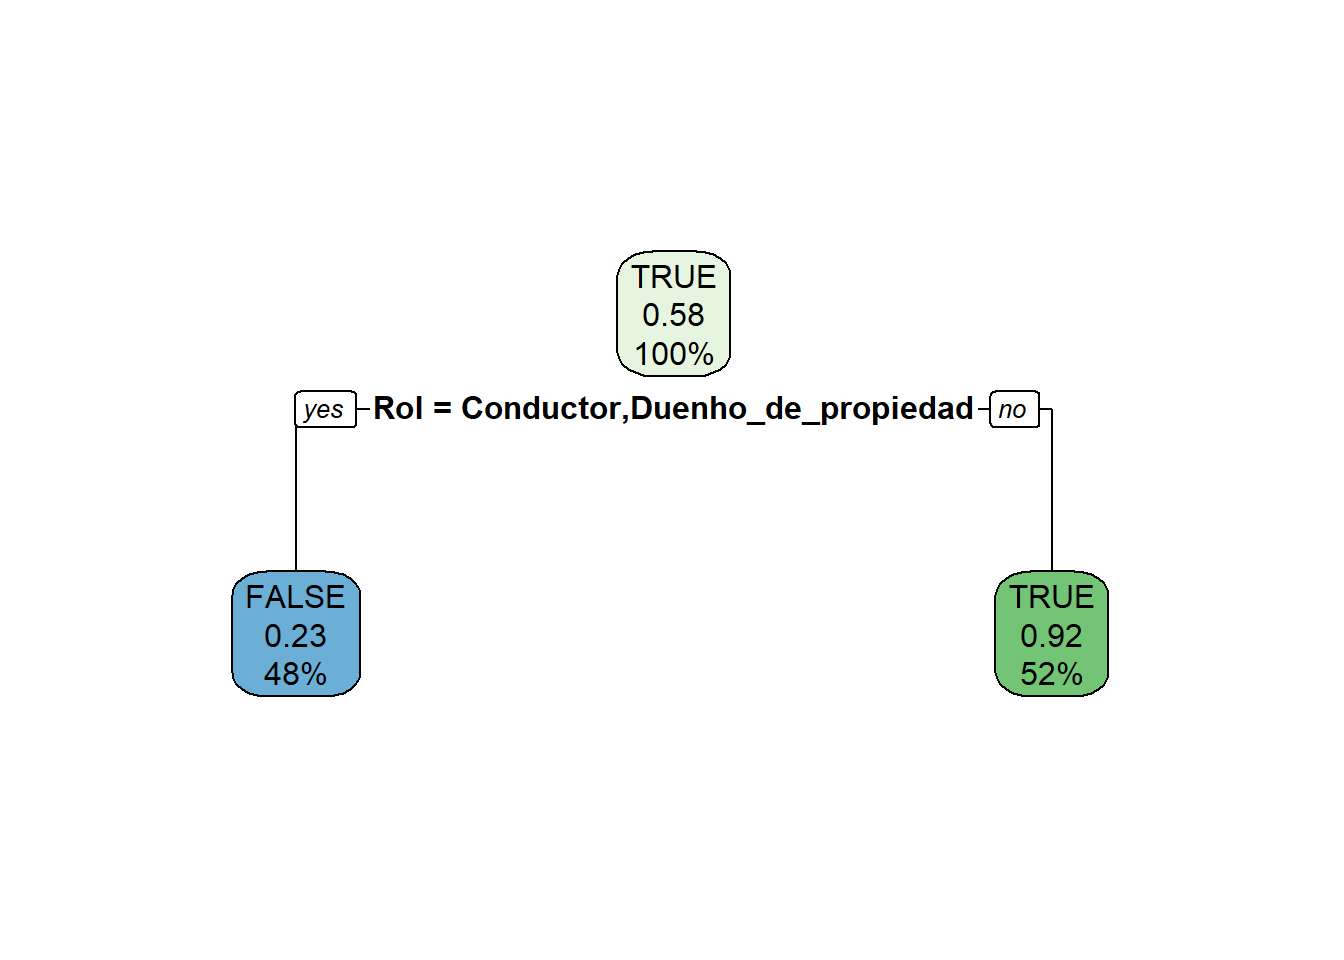
\includegraphics{Regresion_files/figure-latex/unnamed-chunk-15-1.pdf}

\begin{Shaded}
\begin{Highlighting}[]
  \KeywordTok{plot}\NormalTok{(training_data}\OperatorTok{$}\NormalTok{hp, }\KeywordTok{log}\NormalTok{(training_data}\OperatorTok{$}\NormalTok{mpg))}
\end{Highlighting}
\end{Shaded}

\includegraphics{Regresion_files/figure-latex/unnamed-chunk-15-2.pdf}

\begin{Shaded}
\begin{Highlighting}[]
  \KeywordTok{plot}\NormalTok{(}\KeywordTok{log}\NormalTok{(training_data}\OperatorTok{$}\NormalTok{hp), }\KeywordTok{log}\NormalTok{(training_data}\OperatorTok{$}\NormalTok{mpg))}
\end{Highlighting}
\end{Shaded}

\includegraphics{Regresion_files/figure-latex/unnamed-chunk-15-3.pdf}

\begin{Shaded}
\begin{Highlighting}[]
  \KeywordTok{plot}\NormalTok{(training_data}\OperatorTok{$}\NormalTok{weight, training_data}\OperatorTok{$}\NormalTok{mpg)}
\end{Highlighting}
\end{Shaded}

\includegraphics{Regresion_files/figure-latex/unnamed-chunk-16-1.pdf}

\begin{Shaded}
\begin{Highlighting}[]
  \KeywordTok{plot}\NormalTok{(training_data}\OperatorTok{$}\NormalTok{weight, }\KeywordTok{log}\NormalTok{(training_data}\OperatorTok{$}\NormalTok{mpg))}
\end{Highlighting}
\end{Shaded}

\includegraphics{Regresion_files/figure-latex/unnamed-chunk-16-2.pdf}

\begin{Shaded}
\begin{Highlighting}[]
  \KeywordTok{plot}\NormalTok{(}\KeywordTok{log}\NormalTok{(training_data}\OperatorTok{$}\NormalTok{weight), }\KeywordTok{log}\NormalTok{(training_data}\OperatorTok{$}\NormalTok{mpg))}
\end{Highlighting}
\end{Shaded}

\includegraphics{Regresion_files/figure-latex/unnamed-chunk-16-3.pdf}

\begin{Shaded}
\begin{Highlighting}[]
  \KeywordTok{plot}\NormalTok{(training_data}\OperatorTok{$}\NormalTok{disp, training_data}\OperatorTok{$}\NormalTok{mpg)}
\end{Highlighting}
\end{Shaded}

\includegraphics{Regresion_files/figure-latex/unnamed-chunk-17-1.pdf}

\begin{Shaded}
\begin{Highlighting}[]
  \KeywordTok{plot}\NormalTok{(training_data}\OperatorTok{$}\NormalTok{disp, }\KeywordTok{log}\NormalTok{(training_data}\OperatorTok{$}\NormalTok{mpg))}
\end{Highlighting}
\end{Shaded}

\includegraphics{Regresion_files/figure-latex/unnamed-chunk-17-2.pdf}

\begin{Shaded}
\begin{Highlighting}[]
  \KeywordTok{plot}\NormalTok{(}\KeywordTok{log}\NormalTok{(training_data}\OperatorTok{$}\NormalTok{disp), }\KeywordTok{log}\NormalTok{(training_data}\OperatorTok{$}\NormalTok{mpg))}
\end{Highlighting}
\end{Shaded}

\includegraphics{Regresion_files/figure-latex/unnamed-chunk-17-3.pdf}

\begin{enumerate}
\def\labelenumi{\arabic{enumi}.}
\setcounter{enumi}{3}
\tightlist
\item
  Cree un modelo de regresion lineal utilizando el atributo mpg como la
  variable objetivo y en base a las correlaciones observadas en el
  gráfico del punto 2 escoja al menos dos atributos para usarlos como
  variables predictoras para el modelo.
\end{enumerate}

Pista:
\url{https://www.rdocumentation.org/packages/lessR/versions/1.9.8/topics/reg}

Nota: Al crear el modelo utilice el conjunto de datos de entrenamiento
definido en el punto 3.

\begin{Shaded}
\begin{Highlighting}[]
\NormalTok{training_data <-}\StringTok{ }\NormalTok{training_data}

\NormalTok{line_model <-}\StringTok{ }\KeywordTok{lm}\NormalTok{(}\KeywordTok{log}\NormalTok{(mpg) }\OperatorTok{~}\StringTok{ }\NormalTok{hp }\OperatorTok{+}\StringTok{ }\NormalTok{weight, }\DataTypeTok{data =}\NormalTok{ training_data)}
\end{Highlighting}
\end{Shaded}

\begin{Shaded}
\begin{Highlighting}[]
\NormalTok{predicted_data  <-}\StringTok{ }\KeywordTok{predict}\NormalTok{(line_model, test_data)}
\NormalTok{predicts_real <-}\StringTok{ }\KeywordTok{data.frame}\NormalTok{(}\KeywordTok{cbind}\NormalTok{(}\DataTypeTok{real=}\NormalTok{test_data}\OperatorTok{$}\NormalTok{mpg, }\DataTypeTok{predicted =} \KeywordTok{exp}\NormalTok{(predicted_data)))}

\KeywordTok{plot}\NormalTok{(predicts_real)}
\end{Highlighting}
\end{Shaded}

\includegraphics{Regresion_files/figure-latex/unnamed-chunk-19-1.pdf}

\begin{enumerate}
\def\labelenumi{\arabic{enumi}.}
\setcounter{enumi}{4}
\tightlist
\item
  Realice predicciones utilizando el conjunto de pruebas y evalue el
  resultado con la métrica MSE.
\end{enumerate}

\begin{Shaded}
\begin{Highlighting}[]
\KeywordTok{mse}\NormalTok{(predicts_real}\OperatorTok{$}\NormalTok{predicted,predicts_real}\OperatorTok{$}\NormalTok{real)}
\end{Highlighting}
\end{Shaded}

\begin{verbatim}
## [1] 16.10246
\end{verbatim}

\begin{enumerate}
\def\labelenumi{\arabic{enumi}.}
\setcounter{enumi}{5}
\tightlist
\item
  Opcional
\end{enumerate}

6.a Pruebe varios modelos que utilicen diferentes variables y comparar
los resultados obtenidos

6.b Investigar como implementar en R las técnicas de preprocesado y
normalización vistas en clase y aplicarlas a los datos antes de pasarlos
al modelo.


\end{document}
